% --------------------------------------------------------------
% This is all preamble stuff that you don't have to worry about.
% Head down to where it says "Start here"
% --------------------------------------------------------------
 
\documentclass[12pt]{article}
 
\usepackage[nouppercase,headsepline,footsepline,plainfootsepline]{scrpage2}
\automark{section}
\pagestyle{scrheadings}
%\clearscrheadfoot
\ihead{Numerical Sequences and Series}
%\ofoot[\pagemark]{\pagemark}% Optional argument controls chapter-starting pages
\ifoot[(Author)]{{\sl \hfill Meenmo K.}}

\usepackage[margin=1in]{geometry} 
\usepackage{amsmath,amsthm,amssymb,scrextend}
\usepackage{fancyhdr}
\usepackage{enumitem}
\usepackage{amsmath}
\usepackage{amssymb}
\usepackage{textcomp}
\usepackage{fancybox}
\usepackage{tikz}
\usepackage{cancel}
\usepackage{tasks}


\newcommand{\N}{\mathbb{N}}
\newcommand{\Z}{\mathbb{Z}}
\newcommand{\I}{\mathbb{I}}
\newcommand{\R}{\mathbb{R}}
\newcommand{\Q}{\mathbb{Q}}
\renewcommand{\qed}{\hfill$\blacksquare$}
\let\newproof\proof
\renewenvironment{proof}{\begin{addmargin}[1em]{0em}\begin{newproof}}{\end{newproof}\end{addmargin}\qed}
% \newcommand{\expl}[1]{\text{\hfill[#1]}$}
\setlength{\parindent}{0pt}
\newenvironment{theorem}[2][Theorem]{\begin{trivlist}
\item[\hskip \labelsep {\bfseries #1}\hskip \labelsep {\bfseries #2.}]}{\end{trivlist}}
\newenvironment{lemma}[2][Lemma]{\begin{trivlist}
\item[\hskip \labelsep {\bfseries #1}\hskip \labelsep {\bfseries #2.}]}{\end{trivlist}}
\newenvironment{problem}[2][Problem]{\begin{trivlist}
\item[\hskip \labelsep {\bfseries #1}\hskip \labelsep {\bfseries #2.}]}{\end{trivlist}}
\newenvironment{exercise}[2][Exercise]{\begin{trivlist}
\item[\hskip \labelsep {\bfseries #1}\hskip \labelsep {\bfseries #2.}]}{\end{trivlist}}
\newenvironment{reflection}[2][Reflection]{\begin{trivlist}
\item[\hskip \labelsep {\bfseries #1}\hskip \labelsep {\bfseries #2.}]}{\end{trivlist}}
\newenvironment{proposition}[2][Proposition]{\begin{trivlist}
\item[\hskip \labelsep {\bfseries #1}\hskip \labelsep {\bfseries #2.}]}{\end{trivlist}}
\newenvironment{corollary}[2][Corollary]{\begin{trivlist}
\item[\hskip \labelsep {\bfseries #1}\hskip \labelsep {\bfseries #2.}]}{\end{trivlist}}
 
\settasks{
	counter-format=(tsk[r]),
	label-width=4ex
}

\begin{document}
\section{Sequences of Real Numbers}
\begin{block}A sequence is a map from $\mathbb{N}$ to a set. So a sequence of real numbers is a map $x\colon \mathbb{N}\to\mathbb{R}$ where we write $x_n=x(n), (x_n), \{x_n\}, \text{ or } x_1,x_2,...$.\end{block} \\

\begin{block}{\bf Definition} Let $(x_n)$ be a sequence in $\mathbb{R}\colon\; x\in\mathbb{R}$. We say $x_n$ converges to $x$ and write $x_n\to x$ or $\lim\limits_{n\to\infty} x_n = x$ if $\forall\;\epsilon>0, \exists\;N\in\mathbb{N}$ such that $\forall\;n\ge N,\; |x_n-x|<\epsilon$. Then we call $x$ the limit of $(x_n)$.\end{block}

\vspace{1.5\baselineskip}
\begin{block}{\bf Example} 
\begin{enumerate}[label=(\roman*)]
    \item Let $x_n=\frac{1}{n}.$ Show that $x_n\to 0$ as $n\to\infty$.
    \begin{itemize}
        \item Take $\epsilon>0$, and let $N>\frac{1}{\epsilon}$ such that $N\in \mathbb{N}.$
        \item Now, $\forall N\ge N,\; |x_n-0|=|x_n| = \frac{1}{n}\le \frac{1}{N}<\epsilon$.
    \end{itemize}
    
    \item Let $x_n = 1-\frac{1}{n^2}$. show that $x_n\to 1$ as $n\to \infty$.
    \begin{itemize}
        \item Take $\epsilon>0$, and let $N>\frac{1}{\epsilon}$ such that $N\in \mathbb{N}.$
        \item Now, $\forall N\ge N,\; |x_n- 1|=|1-\frac{1}{n^2} -1| = \frac{1}{n^2} \le \frac{1}{N^2} < \epsilon$.
    \end{itemize}
\end{enumerate}
\end{block}

\vspace{1.5\baselineskip}
\begin{block}{\bf Theorem} Let $(x_n)$ in $\mathbb{R}$ such that $x_n\to x$ and $x_n\to y$ then x=y.\end{block}

\vspace{1\baselineskip}
\begin{block}{\sl Proof.} 
\begin{itemize}
    \item Suppose by contradiction that $|x-y|>0$.
    \item Take $\epsilon=\frac{|x-y|}{2}$. Then
    \begin{itemize}
        \item $\exists\;N_1\in\mathbb{N}$ such that for $n\ge N_1,\;|x_n-x|<\epsilon$
        \item $\exists\;N_2\in\mathbb{N}$ such that for $n\ge N_2,\;|x_n-y|<\epsilon$
    \end{itemize}
    \item Let $N= \max(N_1,N_2)$, then $\forall\;n\geN$,
    $$0<|x-y| = |x-x_n+x_n-y| \le |x-x_n|+|x_n-y|<2\epsilon = |x-y|$$
    This contradicts to the initial assumption that $|x-y|>0$.
\end{itemize}
\end{block}

\newpage
\begin{block}{\bf Theorem} (Algebra of Limits) Let $(x_n), (y_n)$ in $\mathbb{R},\; x_n\to x,\; y_n\to y$. Then
\begin{enumerate}[label=(\roman*)]
    \item $x_n+y_n \to x+y,\; cx_n\to cx\;\;\forall c\in\mathbb{R}$
    \item $x_n\times y_n \to xy$
    \item If $y_n$ with $y\neq 0\;\;\forall\;n\in\mathbb{N},\;$then $\frac{x_n}{y_n}\to \frac{x}{y}.$
\end{enumerate}
\end{block}

\vspace{1\baselineskip}
\begin{block}{\sl Proof.}
\begin{enumerate}[label=(\roman*)]
    \item Let $\epsilon >0$. Then 
    \begin{itemize}
        \item $\exists\;N_1\in\mathbb{N}$ such that $\forall\;n\ge N_1,\;|x_n-x|<\frac{\epsilon}{2}$
        \item $\exists\;N_2\in\mathbb{N}$ such that $\forall\;n\ge N_2,\;|y_n-y|<\frac{\epsilon}{2}$
    \end{itemize}
    Let $N=\max(N_1,N_2)$. Then 
    $$\forall\;n\geN,\;|x_n+y_n-(x+y)|\le |x_n-x|+|y_n-y|<\frac{\epsilon}{2}+\frac{\epsilon}{2}=\epsilon$$
    %\item Then $\forall\;n\ge N=\max(N_1,N_2),\;|$
    
    \item $x_ny_n - xy \to 0\;\Leftrightarrow\; x_ny_n\to xy$.
    \item 
\end{enumerate}
\end{block}

\vspace{1\baselineskip}
\begin{block}{\bf Definition} Monotone Sequence: A sequence $(x_n)$ is called
\begin{enumerate}[label=(\roman*)]
    \item {\sl Monotonically Increasing }  if $x_n\le x_{n+1},\;\forall\;n\in\mathbb{N}$
    \item {\sl Monotonically Decreasing }  if $x_n\ge x_{n+1},\;\forall\;n\in\mathbb{N}$
    \item {\sl Monotone } if either (i) or (ii)
    \item {\sl Bounded } if $\exists\;M>0$ such that $|x_n|\le M\;\;\forall\;n\in\mathbb{N}$.
\end{enumerate}

\vspace{1\baselineskip}
\begin{block}{\bf Theorem} Let $(x_n)$ be monotone. Then $(x_n)$ is convergent if and only if $(x_n)$ is bounded.\\

{\sl Proof.}
\begin{itemize}
    \item Suppose $(x_n)$ is bounded, $x_n\le x_{n+1}\;\;\forall\;n\in\mathbb{N}.$
    \item Then $E = \{x_n\;|\;n\in\mathbb{N} \}$ is non-empty and bounded.
    \item So $x=\sup E$ exists in $\mathbb{R}$.
    \item Let $\epsilon>0,$ then $\exists\;N\in\mathbb{N}$ such that $x-\epsilon<x_N\le x$.
    \item Now $x-\epsilon <x_N\le x_n\le x\;\;\forall\;n\ge N$ by monotonicity.
    \item Hence $\forall\;n\ge N,\;|x_n-x|<\epsilon.$
\end{itemize}
{\sl Note. }If a sequence is convergent, then it is bounded.
\end{block}
\end{block}

\newpage
\begin{block}{\bf Definition}\\ Let $(x_n)$ be a sequence. Suppose $(n_k)$ is a sequence in $\mathbb{N}$. Then $(x_{n_k})$ is a {\sl subsequence}.

\vspace{1\baselineskip}
{\bf Proposition}\\ Let $(x_n)$ be a sequence, then $x_n\to x$ if and only if $x_{n_k}\to x$ for all subsequences $(x_{n_k})$ of $(x_n).$

\vspace{1\baselineskip}
{\bf Example} $x_n=(-1)^n$
\begin{itemize}
    \item Let $n_k=2k$ for $k\in\mathbb{N}$. Then $x_{n_k}=1\;\;\forall\;k$, so $x_{n_k}\to 1$.
    \item Now let $n_j = 2_j+1,\;j\in\mathbb{N}$. Then $x_{n_j}\to -1$. 
    \item Hence $(x_n)$ does not converge. 
\end{itemize}

\textbf{Definition}\\
A sequence of real numbers $(x_n)$ converges to $x$ if 
$\forall\;\epsilon > 0\;\exists\;\N\in\mathbb{N}$ such that $\forall\; n \ge \mathbb{N}, \; |x_n - x| < \epsilon$.\\

\textbf{Theorem} (Bolzano-Weierstrass)\\
Any bounded sequence $(x_n)$ in $\mathbb{R}$ has a convergent subsequence.\\

{\sl Proof.}
$$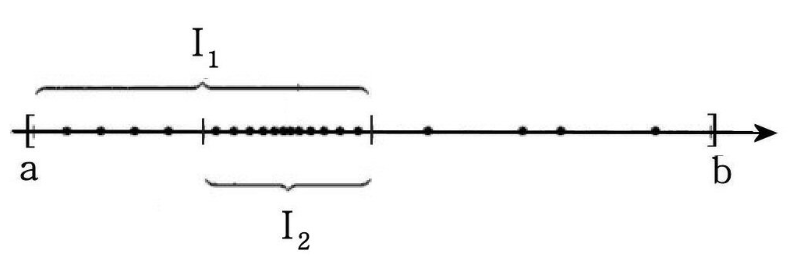
\includegraphics[height=2.7cm, width=13cm]{bolzano.png}$$
\begin{itemize}
    \item Suppose sequence $E = \{x_n\;|\; n \in \mathbb{N}\}$. 
    \item If $E$ is finite, then $\exists$ a subsequence $(x_{n_k})$ such that $x_{n_1}=x_{n_2}=x_{n_3}=\ldots=x_{n_k}=\ldots$ which is convergent.\\
    
    \item On the other hand, suppose $E$ is an infinite sequence.
    \item Now as $E$ is bounded, $\exists\;a<b\in\mathbb{R}$ such that $E\subset[a,b],$ and let $I_0=[a,b]$.
    \item Heine-Borel Theorem, $E$ has a limit point in $[a,b]\subset\mathbb{R}.$\\
    {\sl Recall that since $E$ is a closed and bounded $E$ is compact and has a limit point inside.}
    \item Let the limit point to be $x \in[a,b].$\\
    
    
    \item When $I_0$ is equally divided into two parts, infinitely many $x_n$ must be contained in, at least, one of two parts. Let us call it $I_1$.
    \item Reapting this steps, and we obtain $I_0,I_1,I_2,...\qquad$ i.e. $I_0\supset I_1\supset I_2\supset \ldots$
    
    \item Then choose $n_1\in I_1$, $n_2\in I_2$ such that $n_1<n_2$, $n_3\in I_3$ such that $n_1<n_2<n_3,\;\ldots$
    \item Then $\{x_{n_k}\}$ is a subsequence of $\{x_n\}$, and $x_{n_k}$ and the limit point $x$ are also contained in $I_k$.
    \item Thus we can derive that 
    $|x_{n_k}-x| < \frac{M}{2^k}\hfill$
    (where $M = \frac{b-a}{2}$, so $\frac{M}{2^k}$ is the length of $I_k$).
    \item Since $\lim\limits_{n\to\infty} \frac{M}{2^n} = 0$, this implies that $\lim\limits_{k\to\infty} x_{n_k} = x$
\end{itemize}\\

\vspace{1\baselineskip}
\textbf{Definition}\\
A sequence $(x_n)$ in $\mathbb{R}$ is \textbf{Cauchy} if $\forall\;\epsilon > 0,\; \exists \; N \in \mathbb{N}$ such that $|x_n - x_m| < \epsilon$ if $\forall\;n,m \ge \mathbb{N}$.\\

{\sl Remark.} Cauchy does not require a \underline{known} limit point.\\

\vspace{1\baselineskip}
\textbf{Theorem} $(x_n)$ converges if and only if it is Cauchy.\\

{\sl Proof.}
\begin{itemize}
    \item $\Rightarrow$ Suppose $(x_n)$ converges, $x_n \rightarrow x$. 
    \item Let $\epsilon > 0$. Then $\exists\; N \in \mathbb{N}$ such that $\forall\;n\ge N,\; |x_n - x| < \frac{\epsilon}{2}.$
    \item Now if $n,m \ge N,\; |x_n - x_m| \le |x_n-x|+|x-x_m| < \epsilon.$\\
    
    \item $\Leftarrow$ Suppose $(x_n)$ is Cauchy.
    \item Step 1: $(x_N)$ is bounded.
    \begin{itemize}
        \item $\exists\; n \in \mathbb{N}$, such that $\forall\;n,m \ge N, |x_n-x_m|<1$.
        \item Thus $\forall\;n\ge N,\; |x_n| \le max(|x_n| +1, |x_1|,...,|x_N|)\le M\in\mathbb{R}$. \hfiill i.e. $(x_n)$ is bounded.
    \end{itemize}
    
    \item Step 2: Find the limit.
    \begin{itemize}
        \item By Bolzano-Weierstrass, $\exists$ a subsequence $(x_{n_k})$ such that $(x_{n_k}) \rightarrow x \in \mathbb{R}$.
        \item Let $\epsilon > 0$. Take $N_1 \in \mathbb{N}$ such that $\forall\; k\ge N_1,\; |x_{n_k} - x| <\frac{\epsilon}{2}.$
        \item And by Cauchy condition $\exists\; N_2$, $\forall\; n,m \ge N_2,\; |x_n -x_m| <\frac{\epsilon}{2}.$
        \item $N:= \max\{N_1,N_2\},$ and choose $k$ such that $n_k>N,\;k>N$.
        \item Now if $$n \ge N,\; |x_n -x| \le |x_n-x_{n_k}+x_{n_k}-x|\le |x_n -x_{n_k}| + |x_{n_k} - x|<\frac{\epsilon}{2}+\frac{\epsilon}{2} = \epsilon.\hfill$$ Hence convergent.
    \end{itemize}
\end{itemize}


\newpage
\textbf{Theorem}
\begin{enumerate}[label=(\roman*)]
    \item $\forall\;p>0, \frac{1}{n^p} \rightarrow 0$ as $n \rightarrow \infty$.
    \item $\forall\;x>0, x^{\frac{1}{n}} \rightarrow 1$ as $n \rightarrow \infty$.
    \item $n^{\frac{1}{n}} \rightarrow 1$ as $n \rightarrow \infty$.
    \item $\forall\; p\in \mathbb{R}, x>0, \frac{n^p}{(1+x)^n} \rightarrow 0$.
    \item If $0<x<1, x^n \rightarrow 0$ as $n \rightarrow \infty$.
\end{enumerate}

{\sl Proof.}
\begin{enumerate}[label=(\roman*)]
    \item Exercise
    \item 
    \begin{itemize}
        \item Suppose $x>1$.
        \item By the binomial theorem = $(1+x_n)^n \ge 1+nx_n$.
        \item So $0 < x_n < \frac{x-1}{n} \rightarrow 0$ as $n\rightarrow \infty$.
        \item Hence $x+n \rightarrow 0$. i.e. $x^{\frac{1}{n}} \rightarrow 1$.
        \item In the case(?) $0<x<1, \frac{1}{2} > 1,$ so $\frac{1}{x}^{\frac{1}{n}} \rightarrow 1$.
        \item So $x^{\frac{1}{n}} = \frac{1}{\frac{1}{2}^{\frac{1}{n}}} \rightarrow \frac{1}{1} = 1$
    \end{itemize}

    \item 
    \begin{itemize}
        \item Let $x_n = n^{\frac{1}{n}} -1 \ge 0$
        \item Then $n = (1+x_n)^n \ge \frac{n(n-1)}{2}x_n^2$.
        \hfill (if approach like (ii) not $\to 0$)
        \item So $0 \le x_n \le \sqrt{\frac{2}{n-1}}$ for $n\ge 2$.
    \end{itemize}
    
    
    \item 
    \begin{itemize}
        \item Let $p \in \mathbb{R}, x>0$.
        \item Take $k \in \mathbb{N}$ such that $k > p$.
        \item Suppose $n > 2k$.
        \item Then $(1+x)^n \ge \binom{n}k x^k = \frac{n(n-1)\ldots(n-k+1)}{k!} \ge \frac{n^k}{2^k k!} x^k.$
        \item So $0< \frac{n^p}{(1+x)^n} \le \frac{2^k k!}{x^k} n^{p-k} \rightarrow 0$. 
        \hfill ($p-k<0$ as $k>p$)
    \end{itemize}
    
    
    \item $0<x<1$.
    \begin{itemize}
        \item So $\frac{1}{(1+x)^n} \rightarrow 0$ by (iv). (choose p=0).
        \hfill (where $1+x$ is an arbitrary number)
        \item If $x \in (0,1), \exits\; y>0$ such that $x = \frac{1}{1+y}$.
        \item So $x^n = \frac{1}{(1+y)^n} \rightarrow 0$.
    \end{itemize}
\end{enumerate}

\newpage
\section{Sequences in a metric space}\\
\textbf{Definition}\\
Let $(X,d)$ be a metric space, $(x_n)$ a sequence in $X,\; x \in X$. We say $(x_n)$ converges to $x$ if $\forall\;\epsilon > 0\; \exists\;N\in \mathbb{N}$ such that  $n\ge N$ implying $d(x_n,x) < \epsilon$. We write $x_n \rightarrow x,$ or $\lim\limits_{n\rightarrow \infty} x_n = x$ or $x_n\xrightarrow{d}x$.

\vspace{1\baselineskip}
\textbf{Example}
\begin{enumerate}[label=(\roman*)]
    \item In $\mathbb{R},\; \frac{1}{n} \rightarrow 0$.
    
    \item In $(0,\infty),\; \frac{1}{n}$, however, does not converge.
\end{enumerate}
 
\vspace{1\baselineskip}
\textbf{Theorem}\\
 Let $(X,d)$ be a metric space, $(x_n) \subset X.$
 \begin{enumerate}[label=(\roman*)]
     \item  $x_n \rightarrow x$ if and only if every neighborhood of $x$ contains all, but finitely many of the terms $x_n$.
     \begin{itemize}
         \item $x_n = (-1)^n.\;b_1(1)$ contains infinitely many $x_n$.
         \item $x_n$ does not converge to 1.
     \end{itemize}
     \item If $x\in X, y\in X, x_n \rightarrow x, x_n\rightarrow y, $then $x=y$.
     \item If $(x_n)$ converges, it is bounded.
     \item If $E \subset X$ and $x$ is a limit point of $E$, then $\exists$ a sequence in $(x_n) \subset E$ such that $x_n \rightarrow x$.
 \end{enumerate}
 
 \vspace{1\baselineskip}
 \textbf{Example}
 \begin{itemize}
     \item Take $(\mathbb{R}, d_{disc}).$
$$
 d_{disc}(x,y) =
 \begin{cases}
 1 \text{ if } x \neq y\\
 0 \text{ if } x = y
 \end{cases}
 \hfill (disc \text{ refers to discrete})$$
 
 \item Consider $x_n = \frac{1}{n}.$
 \item Note $d(x_n,0) = 1\;\; \forall\; n$ . So $\{{x_n}\} \subset B_2(0);$ hence ($x_n$) is bounded. 
 \item But if $x\in \mathbb{R}, $ eventually, $x_n \neq x\;\; \forall\; n$
 \hfill (all $x$ are distinct)
 \item so $d(x_n, x) = 1 \;\;\forall\;n.$ 
 \item So $x_n \nrightarrow x\;\;\forall\;x\in\mathbb{R}$\hfill
 i.e. It does not converge.
\end{itemize}
\end{block}
 
\newpage
\begin{block}{\bf Definition}\\
Let $(X,d)$ be a metric space, $(x_n)\subset X$. We say $x_n\to x \in X$ if and only if $\forall\;\epsilon>0,\;\exists\;N\in\mathbb{N}$ such that $\forall\;n\geN,\;d(x_n,x)<\epsilon.$

\vspace{1\baselineskip}
{\bf Theorem} Let $(X,d)$ be a metric space $(x_n)\subset X,\;x\in X$.
\begin{enumerate}[label=(\roman*)]
    \item $x_n\to x$ if and only if every neighborhood of $x$ contains all but finitely many $x_n$.
    \item If $x_n\to x$ and $x_n\to y,$ then $x=y$.
    \item If $(x_n)$ is convergent, it is bounded.
    \item If $E\subset X,\;x$ is a limit point of $E,\;\exists\;(x_n)\subset E$ such that $x_n\to x$.\\
\end{enumerate}

{\sl Proof.}
\begin{enumerate}[label=(\roman*)]
    \item 
    \begin{itemize}
        \item Suppose $x_n\to x.$ Let $r>0,$ and consider $B_r(x).$
        \item Then $\exists\;N\in\mathbb{N}$ such that $\forall\;n\ge N,\;d(x_n,x)<r.\hfill$ i.e. $\forall\;n\ge N,\;x_n\in B_r(x)$
        \item So the only parts $x_n$ that could be outside $B_r(x)$ are $x_1,\ldots,x_{N-1}$ which is finite.\\
    \end{itemize}
    {\sl The other way}
    \begin{itemize}
        \item Suppose every neighborhood of $x$ contains all but finitely many $x_n$.
        \item Let $\epsilon>0$. Then $\exists\;N\in\mathbb{N}$ such that $\forall\;n\ge N,\;x_n\in B_\epsilon(x).$ 
        \item i.e. $\forall\; n\ge N,\;d(x_n,x)<\epsilon$.
    \end{itemize}
    
    \item Exercise
    \item 
    \begin{itemize}
        \item Suppose $x_n\to x$. Then $\exists\;N\in\mathbb{N}$ such that $\forall\;n\ge N,\;d(x_n,x)<1$.
        \item Let $M=\max(d(x_1,x),\ldots,d(x_N,x), 1).$
        \item Then $\forall\;n\in\mathbb{N},\;d(x_n,x)<M.$
        \item So $\forall\;n\in\mathbb{N},\;x_n\in B_M(x)$. Hence bounded.
    \end{itemize}
    
    \item 
    \begin{itemize}
        \item Since $x$ is a limit point, $\exists\; x_1\in E\cap B_1(x)$.
        \item In fact, for any $n\in \mathbb{N},\;\exists\;x_n\in E\cap B_\frac{1}{n} (x).$
        \item Then $d(x_n,x)<\frac{1}{n}\;\;\forall\;n$. So $x_n\to x$.
        \item Let $\epsilon >0,$ take $N>\frac{1}{\epsilon}\Leftrightarrow 1<\epsilon N.$  (By Archimedean property, $\exists\; N$ s.t. $1<\epsilon N$) 
        \item Then $n\ge N,\; d(x_n,x)<\frac{1}{n}\le \frac{1}{N}<\epsilon$; hence $(x_n)\subset E$.
    \end{itemize}
\end{enumerate}

\vspace{1\baselineskip}
{\sl Note.} $E=\{x\}\subset X$\\
The sequence $x_n = x\;\;for\;n$ is such that $x_n\to x,\;(x_n)\subset E,$ but $E$ has no limit points ($E$ finite). i.e. $x$ is not a limit point.
\end{block} 

\newpage
{\bf Theorem} In $\mathbb{R}^k,$ let $(x_n)\subset \mathbb{R}^k$, write $x_n = (x_n^1,\ldots, x_n^k).$
\begin{enumerate}[label=(\roman*)]
    \item $x_n\to x = (x^n,\ldots, x^n)$ if and only if $x_n^j\to x^j\;\;\forall\;j=1,\ldots,n$
    \item Let $(x_n), (y_n)$ be sequences of $\mathbb{R}^k.$\quad i.e. $(x_n),(y_n)\subset \mathbb{R}^k,$
    $$(\beta_n)\subset \mathbb{R},\;x_n\to x,\;y_n\to y,\; \beta_n\to \beta \text{, then }    x_n+y_n \to x+y,\;\beta_n x_n\to \beta x$$
\end{enumerate}
{\sl Proof.}
\begin{enumerate}[label=(\roman*)]
    \item 
    \begin{itemize}
        \item Suppose $x_n\to x.$ Then $\forall\;j\in \{1,\ldots,k\},\; |x_n^j - x^j| \le |x_n-x| \to 0$
        \item Now, suppose $x_n^j\to x^j.$ Let $\epsilon >0,$ for each $j=1,\ldots,k$.
        \item Then $\exists\;N_j\in\mathbb{N}$ such that $\forall\;n\ge N_j,\;|x_n^j-x^j|<\frac{\epsilon}{\sqrt{k}}$
        \item $N:= \max(N_1,\ldots,N_k)$, then
        $$\forall\; n\ge N,\;|x_n-x|=\left(\sum_{j=1}^k |x_n^j - x^j|\right)^{1/2} < \left(\sum_{j=1}^k \frac{\epsilon^2}{k}\right)^{1/2} =\epsilon$$
    \end{itemize}
    \item Exercise.\\
\end{enumerate}

{\bf Theorem} Let $(X,d)$ be compact. Then if $(x_n)\subset X,\;\exists$ a convergent subsequence $(x_{n_k}).$
{\sl Proof.}
\begin{itemize}
    \item Let $E=\{x_n\;|\;n\in\mathbb{N}\}$
    \item If $E$ is finite, then $\exists$ a $x\in E$ and a sequence $\{n_k\}$ with $n_1<n_2<n_3<\ldots,$ such that $$x_{n_1}=x_{n_2}=\ldots = x$$
    The subsequence$\{x_{n_k}\}$ so obtained converges evidently to $x$.\\
    
    \item If $E$ is infinite which is a subset of a compact set $X$, then $E$ has a limit point $x\in X$. (Theorem 2.37 on Rudin)
    \item Choose $n_1$ so that $d(p,p_{n_1})<1$. 
    \item Having chosen $n_1,\ldots,n_{k-1},$ there is an integer $n_k>n_{k-1}$ such that $d(p,p_{n_k})< \frac{1}{k}.$\\ 
    {\sl (By the Theorem 2.20 on Rudin: 
    If $p$ is a limit point of a set $E$, then every neighborhood of $p$ contains infinitely many points of $E$.)}
    \item Then $\{x_{n_k}\}$ converges to $x$.
\end{itemize}

\newpage
{\bf Theorem}\\The subsequential limits of a sequence $\{x_n\}$ in a metric space $X$ form a closed subset of $X$.


{\sl Proof.}
\begin{itemize}
    \item Let $E^*$ be the set of all subsequential limits of $\{x_n\}$ and let $y$ be a limit point $E^*$.\\ We have to show that $y\in E^*.$
    \item Choose $n_1$ so that $x_{n_1}\neq y$, and $\delta = d(x_{n_1},y)>0.$
    \item Suppose $n_1,...,n_{k-1}$ are chosen.
    \item Since $y$ is a limit point of $E^*$, there is an $x\in E^*$ with $d(x,y)<\frac{\delta}{2^k}$
    \item Now $x\in E^*$ which is a subsequential limit.
    \item As $x\in E^*,\; \exists\; n_{k-1}<n_k$ such that $d(x_{n_k},x)<\frac{\delta}{2^k}$
    \item Now $d(x_{n_k}, y)\le d(x_{n_k},x)+d(x,y)<2^{-k+1}\delta \to 0$. Hence convergent.
    \item So $x_{n_k}\to y.$ Hence $y\in E^*$, and further $E^*$ is closed. 
\end{itemize}

{\bf Remark} In general metric space, Cauchy does not imply convergence.

\vspace{1\baselineskip}
{\bf Theorem}
\begin{enumerate}[label=(\roman*)]
    \item In any metric space $X$, every convergent sequence is a Cauchy sequence.
    \item If $X$ is a compact metric space and if $\{p_n\}$ is a Cauchy sequence in $X$, then $\{p_n\}$ converges to some point of $X$.
    \item In $\mathbb{R}^k$, every Cauchy sequence converges.
\end{enumerate}

\vspace{1\baselineskip}
{\bf Definition} \\
Let $E\subset X$. We definte the \underline{diameter} of $E$ to be diam$(E) = \sup\{d(x,y)\;|\; x,y\in E\}$\\

{\sl Note.}
\begin{itemize}
    \item If $(x_n)$ is a sequence, write $E_N=\{x_N, x_{N+1},...\},$\\ 
    then $(x_n)$ is Cauchy if and only if $\text{diam}(E_N) \to 0.\hfill (\epsilon>0,\; \text{diam}(E_N) <\epsilon)$
    \item $\text{diam}(E_N)$ maybe infinite.\\
\end{itemize}

{\bf Theorem}
\begin{enumerate}[label=(\roman*)]
    \item Let $E\subset X$. Then diam$(E)$ = diam ($\overline{E}$).
    \item Let $(K_n)\subset X$ be a sequence of compact sets such that $K_{n+1}\subset K_n$, and diam$(K_n)\to 0$ as $n\to \infty$, then non-empty $K= \bigcap\limits_{n=1}^\infty K_n$ is a single point.
\end{enumerate}

\newpage
{\sl Proof.}
\begin{enumerate}[label=(\roman*)]
    \item 
    \begin{itemize}
        \item It is clear that diam($E)\le$ diam($\overline{E}$).
        \item We prove $\forall\;\epsilon>0,\;\text{diam}\overline{E}<2\epsilon +\text{diam}(E)$.
        \item Let $\overline{x},\overline{y}\in \overline{E},\; \epsilon>0,$ and $x,y\in E$ such that $d(x,\overline{x})<\epsilon,\;d(y,\overline{y})<\epsilon$
        \item Then $d(\overline{x},\overline{y})\le d(\overline{x},x) + d(x,y)+d(y,\overline{y}) < 2\epsilon + \text{diam}(E)$
        \item Now take sup over $\overline{x},\overline{y}\in \overline{E}$: $ \sup\{d(\overline{x},\overline{y})\;|\; x,y\in E\}= $ diam$(\overline{E})$ 
        \\ $\Rightarrow$ diam$(\overline{E})\le 2\epsilon +$diam($E)$.
        \item As $\epsilon>0$ is arbitrary, this gives diam($\overline{E})\le \text{diam}(E)$
        \item Thus we proved diam($E$) = diam($\overline{E}$)\\
    \end{itemize}
    
    \item
    \begin{itemize}
        \item Note that $K\neq \phi$ by the theorem in Compact Sets.
        \item Also $\forall n\; K\subset K_n,$ so $0\le$ diam$(K)\le$ diam $(K_n) \to 0$. Hence diam$(K)$=0.
        \item Suppose $K$ has more than one point. Then $\exists\; x\neq y$ such that $x,y\in K$. 
        \item Hence $0<d(x,y)\le$ diam$(K)$\\
    \end{itemize}
\end{enumerate}

{\bf Theorem}
\begin{enumerate}[label=(\roman*)]
    \item If $(x_n)$ is convergent, then $(x_n)$ is a Cauchy sequence.
    \item Suppose $X$ is compact. Then $(x_n)$ is a Cauchy sequence; so $(x_n)$ is convergent.
    \item In $\mathbb{R}^n,\;\text{if }(x_n)$ is a Cauchy sequence, then $(x_n)$ is convergent.\\
\end{enumerate}

{\sl Proof.}
\begin{enumerate}[label=(\roman*)]
\item
\begin{itemize}
    \item Let $\epsilon>0$, and suppose $x_n\to x\in X$.
    \item Then $\exists\; N\in\mathbb{N},$ such that if $n\ge N,\; d(x_n,x)<\frac{\epsilon}{2}$
    \item Then if $n,m\ge N,\; d(x_n,x_m)\le d(x_n,x)+d(x,x_m)<\epsilon$
\end{itemize}

\item 
\begin{itemize}
    \item Suppose $(x_n)$ is Cauchy. Let $E_N= \{x_n\;|\;n\ge N\}$, then diam($E_N) \to 0$ as $N\to\infty$.
    \item Clearly for each $n,\; E_n\subset \overline{E}_n$ and $E_{n+1}\subset E_n$.
    \item Thus $\overline{E}_{n+1} \subset \overline{E}_n$. As $X$ is compact and $\overline{E}_n$ is closed, $\overline{E}_n$ is compact.
    \item Further, diam$(\overline{E}_n)$ = diam($E_n)\to 0$. Thus $\bigcap\limits_{n=1}^\infty \overline{E}_n = \{x\}$ for some $x\in X$.
    \item Let $\epsilon >0$. Then $\exists\;N\in\mathbb{N}$ such that $\forall\;n\geN,$ diam($\overline{E}_n)<\epsilon$.
    \item Also, $x\in\overline{E}_n$ for all $n\in\mathbb{N}$.
    \item So if $y\in E_n,\; n\ge N,$ we have $y\in \overline{E}_n$, hence $d(x,y)\le \text{diam}(\overline{E}_n) <\epsilon$.
    \item i.e. if $n\ge N,\;x_n\in E_n,$ so $d(x,x_n)<\epsilon,$ so $x_n\to x$.
\end{itemize}
\item Exercise.
\end{enumerate}

\newpage
{\bf Definition} A metric space $(X,d)$ is called \underline{complete} if every Cauchy sequence in $X$ converges to a point in $X$.\\

{\bf Example}
\begin{itemize}
    \item $\mathbb{R}^n$ is complete.
    \item If $X$ is compact, then $X$ is complete.
    \item If $X$ is complete and $Y\subset X$ is closed, then $Y$ is complete.
\end{itemize}

\section{Limit Superior \& Inferior}
{\bf Definition} Let $(x_n)$ be a sequence of real numbers.
\begin{itemize}
    \item $x_n\to\infty$ if $\forall\;M>0,\;\exists\;N\in\mathbb{N}$ such that $\forall\;n\ge N,\;M<x_n$.
    \item $x_n\to -\infty$ if $\forall\;M>0,\;\exists\;N\in\mathbb{N}$ such that $\forall\;n\ge N,\;x_n<-M$.\\
\end{itemize}

{\bf Theorem} Suppose $x_n\to \infty,\;y_n\to\infty,\; c>0$
\begin{tasks}(2)
\task $x_n+y_n\to \infty,\; cx_n\to\infty$
\task $-x_n\to-\infty$
\end{tasks}

\vspace{1\baselineskip}
{\bf Theorem} suppose $x_n\to \infty, (y_n)$ is bounded.
\begin{itemize}
    \item Then $x_n+y_n\to \infty$
    \item If $x_n\to\infty$ and $\exists\;N_0\in\mathbb{N}\;\;\forall\;n\ge N_0,\; y_n\ge x_n,$ then $y_n\to\infty$\\
\end{itemize}

{\bf Definition} Let $(x_n) \subset \mathbb{R}$. We define the \underline{limit superior} of $(x_n)$ to be $$\limsup\limits_{n\to\infty} x_n = \lim\limits_{n\to\infty}\left(\sup\limits_{n\le k} x_k\right)$$
{\sl Note.} 
\begin{itemize}
    \item $\left(\sup\limits_{n\le k}x_k\right)$ is monotonically decreasing sequence.
    \item $\limsup\limits_{n\to\infty} x_n$ always exists in $\overline{\mathbb{R}}$.
\end{itemize}

We define the \underline{limit inferior} as 
$$\liminf\limits_{n\to\infty} x_n = \lim\limits_{n\to\infty}\left(\inf\limits_{n\le k} x_k\right)$$
*This always exists in $\overline{\mathbb{R}}$.

\newpage
{\bf Theorem} Let $(x_n)\subset \mathbb{R}$. Let $E$ be the set of limits of subsequences of $(x_n)$, so $E\subset \mathbb{R}$.
\begin{enumerate}[label=(\roman*)]
    \item $\limsup\limits_{n\to \infty} x_n = \sup E,\; \liminf\limits_{n\to\infty} x_n = \inf E$
    \item $\limsup\limits_{n\to\infty} x_n,\; \liminf\limits_{n\to\infty} x_n \in E$
    \item If 
    \begin{cases}
    $x \textgreater\; \limsup\limits_{n\to\infty} x_n,\;\exists\; N\in\mathbb{N}$ such that $\forall\; n\le N,\; x_n<x$\\
    $x \textless\; \liminf\limits_{n\to\infty} x_n,\;\exists\; N\in\mathbb{N}$ such that $\forall\; n\le N,\; x_n<x$
    \end{cases}
    \item $\limsup\limits_{n\to\infty} x_n$ is the only element of $E$ such that (iii) holds.
\end{enumerate}

{\sl Proof}
\begin{enumerate}[label=(\roman*)]
    \item Suppose $\limsup\limits_{n\to\infty} x_n\in\mathbb{R}$
    \begin{itemize}
        \item Step 1: $\sup E\le \limsup\limits_{n\to\infty} x_n$
            \begin{itemize}
                \item Let $\epsilon >0$. Then $\exists\;N\in\mathbb{N}$ such that $\forall\; n\ge N\;\;\sup\limits_{k\ge n} x_k < \limsup\limits_{n\to\infty} x_n +\epsilon$
                
                \item Hence $x\le \limsup\limits_{n\to\infty} x_n + \epsilon$ 
                \item As $\epsilon>0$ is arbitrary (any positive number), $\sup E\le \limsup\limits_{n\to 0} x_n$
            \end{itemize}
       
        \item Step 2: $\limsup\limits_{n\to\infty} x_n \le \sup E$
            \begin{itemize}
                \item Let $\epsilon >0.$ Now $\exists\;x\in E$ such that $\sup E -\epsilon < x\le \sup E$
                \item Then $\exists$ a subsequence $x_{n_k}\to x$
                \item So $\exists\; N\in\mathbb{N}$ such that $\forall\; k\ge N,\; x_{n_k} >x-\epsilon$
                \item In particular, $\sup\limits_{k\ge n} x_k \ge \sup\limits_{j\ge n_k} x_{n_k} > x-\epsilon > \sup E - 2\epsilon$
                \item Hence $\limsup\limits_{n\to\infty} x_n \ge \sup E - 2\epsilon$. So $\sup E\le \limsup\limits_{n\to\infty} x_n$
            \end{itemize}
        
        \item Step 3
        \begin{itemize}
            \item Let $\epsilon >0.$ Suppose $\limsup\limits_{n\to\infty} x_n > \sup E$. Choose $\epsilon=\frac{\limsup\limits_{n\to\infty} x_n - \sup E}{2}$
            \item Then $\exists\; N\in\mathbb{N}$ such that $\forall\;n\ge N,\;\sup\limits_{k\ge n}x_k > \limsup\limits_{n\to\infty} x_n - \frac{\epsilon}{2}$
            \item Choose a subsequence for each $k=1,2,3,\ldots$.
            \item Let $x_{n_k}$ be such that $x_{n_k} > \sup\limits_{j\ge k} x_j - \frac{\epsilon}{2} > \limsup\limits_{n\to\infty} x_n -\epsilon$
            \item So as $x_{n_k}$ is bounded below, $\exists$ a further subsequence $x_{n_{k_j}}$ such that either $x_{n_{k_j}}\to x,$ or $x_{n_{k_j}}\to \infty$.
            \item Then if $x_{n_{k_j}}\to x,$ we have $x\ge \limsup\limits_{n\to\infty} x_n - \epsilon$
            \item But then 
            \begin{align}
                x&\ge \limsup\limits_{n\to\infty} x_n - \epsilon \nonumber \\
                &=\limsup\limits_{n\to\infty} x_n - \frac{\limsup\limits_{n\to\infty} x_n - \sup E}{2}\nonumber \\ 
                &=\frac{\limsup\limits_{n\to\infty} x_n +\sup E}{2} > \sup E \nonumber            \end{align}
        
        \end{itemize}
        \item Or $x_{n_{k_j}} \to \infty$, then $\infty\in E,$ but $\sup E<\limsup\limits_{n\to\infty} x_n <\infty$
        \item But those are in contradiction as $x\in E$.
        \item So $\limsup\limits_{n\to\infty} x_n \le \sup E$. Thus $\limsup\limits_{n\to\infty} x_n = \sup E$.
    \end{itemize}

    \item 
        \begin{itemize}
            \item Suppose $\limsup\limits_{n\to\infty} x_n = \infty$. Then $\sup\limits_{k\ge n} x_k = \infty\;\;\forall\;n\in\mathbb{N}$
            \item So $\exists\; x_{n_k}\to \infty,$ hence $\infty\in E$.
            \item Suppose $\limsup\limits_{n\to\infty} x_n \in\mathbb{R}$. Then $E\neq \phi$, bounded above.
            \item We know that $E$ is closed since  a set of subsequential limits is closed. So $\sup E\in E$ from (i) $\limsup\limits_{n\to\infty} x_n = \sup E$.\\
            
            \item Suppose $\limsup\limits_{n\to\infty} x_n =-\infty$
            \item So $\sup\limits_{k\ge n} x_k\to -\infty$ as $n\to \infty$. Hence if $M>0$, then $\exsits\;N\in\mathbb{N}$ such that $$\forall\; n\ge N\;\;\sup\limits_{k\ge n} x_n <-M$$
            \hfill i.e. $\sup\limits_{n\ge N} x_n < -M$
            \item So $\forall\;n\ge N,\; x_n <-M$. Hence the sequence itself $x_n\to -\infty$. So $-\infty \in E$.
        \end{itemize}
        
    \item 
    \begin{itemize}
        \item Let $x>\limsup\limits_{n\to\infty} x_n$ and take $\epsilon = \frac{x-\limsup\limits_{n\to\infty} x_n}{2}.$
        \item As $\sup\limits_{k\ge n} x_k < \limsup\limits_{n\to\infty} x_n,\; \exists\; N\in\mathbb{N}$ such that $\forall\;n\ge N,\; \sup\limits_{k\ge n} x_k < \limsup\limits_{n\to\infty} x_n + \epsilon$
        \item So $\forall\;n\ge N,\;x_n < \limsup\limits_{n\to\infty} x_n+\epsilon = \limsup\limits_{n\to\infty} x_n +\frac{\left(x-\limsup\limits_{n\to\infty} x_n\right)}{2} = \frac{x+\limsup\limits_{n\to\infty} x_n}{2}<x$
    \end{itemize}
    
    \item
    \begin{itemize}
        \item Let $x,y\in E$ such that $x<y$ and $x,y$ satisfying (iii). Take $z\in(x,y)$.
        \item Applying (iii) with $x$ and $z,\;\exists\;N\in\mathbb{N}$ such that $\forall\; n \ge N,\;x_n<z<y$
        \item But as $y\in E,\;\exists$ a subsequence $x_{n_k}\to y$
        \item So $\exists\; \widetilde{N}\in\mathbb{N}$ such that $\forall\;k\ge \wildtilde{N},\;x_{n_k}>z.$
        \item This proof is incomplete
    \end{itemize}
\end{enumerate}


%{\bf Theorem} Suppose $(x_n),\; (y_n)\subset\mathbb{R}$ such that $\exists\;N$
\end{document}